\documentclass{article}

\usepackage{graphicx}
\usepackage{tikz}
\usepackage{tikzsymbols}
\usetikzlibrary{calc,patterns,shapes.geometric}
\pagestyle{empty}
\usepackage[margin=0pt]{geometry}
\geometry{papersize={14in,12in}}

\def\centerarc[#1](#2)(#3:#4:#5){\draw[#1] ($(#2)+({#5*cos(#3)},{#5*sin(#3)})$) arc (#3:#4:#5);}

\begin{document}
	\begin{figure}
		\centering
		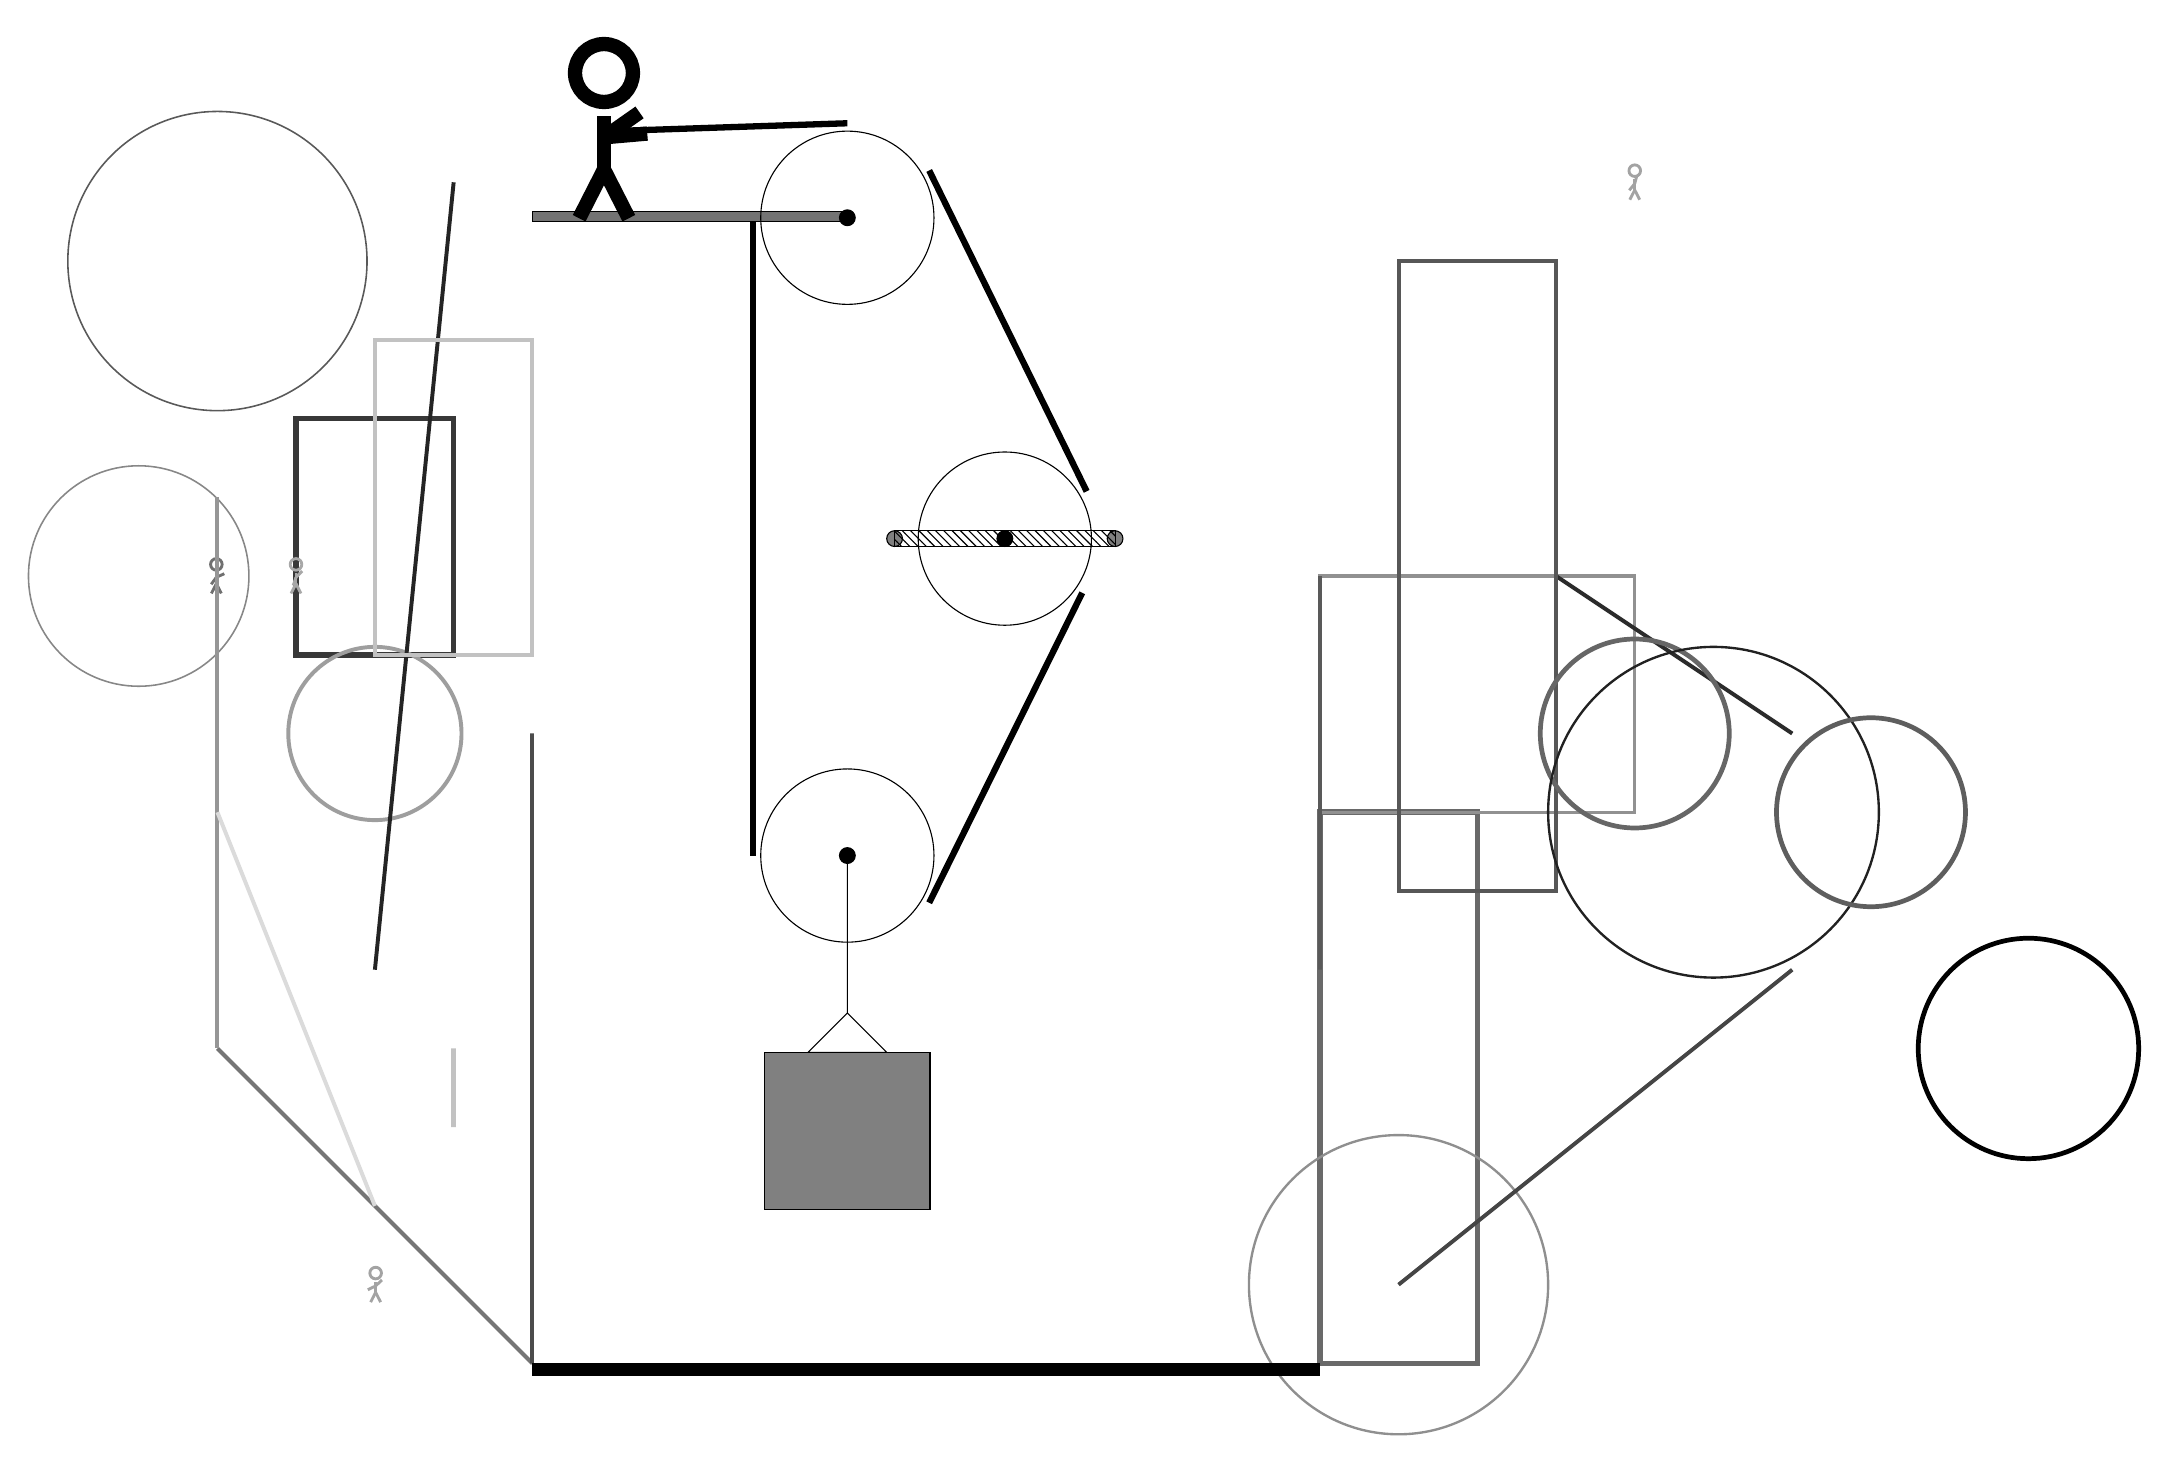
\begin{tikzpicture}
			%%%%% START %%%%%
			
			\draw[fill=black!55] (-2, 11.5) rectangle (2, 11.625);
			
			\draw (2, 3.45) circle (1.1);
			\draw[fill=black] (2, 3.45) circle (0.1);
			
			\draw (2, 11.55) circle (1.1);
			\draw[fill=black] (2, 11.55) circle (0.1);
			
			\draw[fill=white](4, 7.475) circle (1.1);
			\draw[fill=black] (4, 7.475) circle (0.1);
			\draw[fill=black!50] (2.6, 7.475) circle (0.1);
			\draw[fill=black!50] (5.4, 7.475) circle (0.1);
			\draw[pattern=north west lines, pattern color=black] (2.6, 7.575) rectangle (5.4, 7.375);
			
			\draw (2, 3.45) -- (2, 1.45) -- (1.5, 0.95) -- (2.5, 0.95) -- (2, 1.45);
			\draw[fill=black!50] (0.95, 0.95) rectangle (3.05, -1.05);
			
			\draw[line width=0.7mm, color=black!78] (-3, 9) rectangle (-5, 6);
			
			\draw[line width=0.7mm, color=black!59] (10, 4) rectangle (8, -3);
			\draw[line width=0.4mm, color=black!43] (8, 7) rectangle (12, 4);
			\draw[line width=0.5mm, color=black!54](-6, 1) -- (-2, -3);
			\draw[line width=0.5mm, color=black!65] (8, 2) rectangle (8, 7);
			\node[line width=0.5mm, color=black!36] at (12, 12) {\Strichmaxerl[2][51][75]};
			\draw [line width=0.3mm, color=black!44](9, -2) circle (1.9);
			
			\node[line width=0.2mm, color=black!56] at (-6, 7) {\Strichmaxerl[2][54][24]};
			\node[line width=0.6mm, color=black!34] at (-5, 7) {\Strichmaxerl[2][71][45]};
			\draw [line width=0.2mm, color=black!47](-7, 7) circle (1.4);
			\draw[line width=0.5mm, color=black!41](-6, 8) -- (-6, 1);
			\draw[line width=0.6mm, color=black!24] (-3, 0) rectangle (-3, 1);
			\draw[line width=0.5mm, color=black!73](9, -2) -- (14, 2);
			
			\draw[line width=0.5mm, color=black!83](11, 7) -- (14, 5);
			\draw[line width=0.5mm, color=black!66] (9, 3) rectangle (11, 11);
			\draw [line width=0.5mm, color=black!38](-4, 5) circle (1.1);
			
			\draw[line width=0.5mm, color=black!70] (-2, 5) rectangle (-2, -3);
			\draw [line width=0.6mm, color=black!60](12, 5) circle (1.2);
			\node[line width=0.5mm, color=black!36] at (-4, -2) {\Strichmaxerl[2][26][43]};
			\draw [line width=0.2mm, color=black!65](-6, 11) circle (1.9);
			\draw[line width=0.5mm, color=black!86](-3, 12) -- (-4, 2);
			
			\draw[line width=0.5mm, color=black!14](-4, -1) -- (-6, 4);
			\draw[line width=0.5mm, color=black!24] (-4, 10) rectangle (-2, 6);
			\draw [line width=0.3mm, color=black!87](13, 4) circle (2.1);
			\draw[line width=0.6mm, color=black!33] (-4, 5) rectangle (-4, 5);
			
			\draw [line width=0.6mm, color=black!100](17, 1) circle (1.4);
			\draw [line width=0.6mm, color=black!63](15, 4) circle (1.2);
			
			\draw[line width=0.8mm] (0.8, 11.5) -- (0.8, 3.45);
			\centerarc[line width=0.8mm](2, 3.45)(180:330:1.2000000000000002);
			\draw[line width=0.8mm](3.0392, 2.85) -- (4.983, 6.7867);
			\centerarc[line width=0.8mm](4, 7.475)(390:325:1.2000000000000002);
			\draw[line width=0.8mm](5.0392, 8.075) -- (3.0392, 12.15);
			\centerarc[line width=0.8mm](2, 11.55)(30:90:1.2000000000000002);
			\draw[line width=0.8mm](2, 12.75) -- (-1, 12.65);
			
			\node at (-1, 12.65) {\Strichmaxerl[10][-175][35]};
			
			\draw[fill=black] (-2, -3) rectangle (8, -3.15);
			
			%%%%% END %%%%%
		\end{tikzpicture}
	\end{figure}	
\end{document}